% Advisor report: the grid-scale structure in the AMOC adjoint's heat- and freshwater-flux sensitivities, state as of
% 28 November 2026. Build with `latexmk -pdf omip_amoc_adjoint_advisor_report_20261128.tex` in this directory.
% Detail: findings 16-31 of the repository-root LOGBOOK.md; previous report omip_amoc_adjoint_advisor_report.tex.
\documentclass[10pt]{article}

\usepackage[margin=0.8in]{geometry}
\usepackage{amsmath, amssymb}
\usepackage{booktabs}
\usepackage{graphicx}
\usepackage{hyperref}
\usepackage{siunitx}
\usepackage{enumitem}
\usepackage{caption}
\usepackage{float}
\usepackage{titlesec}
\titlespacing*{\section}{0pt}{9pt}{3pt}
\titlespacing*{\subsection}{0pt}{6pt}{2pt}
\setlist{nosep, leftmargin=1.3em}
\captionsetup{font=small, skip=4pt}
\setlength{\parskip}{4pt}
\setlength{\parindent}{0pt}

\newcommand{\gvec}{\mathbf{g}}

\title{\vspace{-2em}\textbf{The checkerboard in the AMOC adjoint's surface-flux sensitivities}\\[2pt]
       \large Progress report\vspace{-0.4em}}
\date{28 November 2026\vspace{-1em}}

\begin{document}
\maketitle

\section{Summary}

The last report (20 November) showed Pillar-style lead-time maps whose heat- and freshwater-flux columns carried a
cell-scale checkerboard, and said they should not be interpreted yet. This report explains that structure and
removes it from the controls.
\begin{enumerate}
  \item \textbf{The checkerboard is real.} It is not an adjoint error: finite differences along its grid-scale part
        agree with the frozen-CATKE adjoint to \SIrange{0.3}{3}{\percent} in stable columns, at \ang{2} and \ang{1}.
        The wind-stress sensitivities look smooth only because the stress is interpolated to cell faces, which removes
        the alternating components by construction.
  \item \textbf{Differentiating CATKE is wrong, so the frozen adjoint is the one to use.} With CATKE differentiated,
        the adjoint is exact for about 120 steps (10 days) and then wrong. The cause is one cell at the mixed-layer
        base where the turbulent kinetic energy sits at its floor.
  \item \textbf{It lives in four places}: the dipole along the section line, the corners of the section's staircase,
        one- to two-cell-wide paths along the coasts, and a row-to-row stripe in convecting columns. The stripe
        appears at both \ang{2} and \ang{1}. Averaging the objective over a \ang{3} band removes the corners but not
        the stripe.
  \item \textbf{Smoothed flux controls remove it.} The fluxes are written as $Q = Q_0 + S c$, with $S$ two passes of a
        1-2-1 filter. The gradient with respect to $c$ is exactly $S^{\mathsf T}\gvec$. Its grid-scale share falls to
        that of the wind stress (Figs.~\ref{fig:lead-raw}, \ref{fig:lead-smooth}).
  \item \textbf{The smoothed gradient is accurate.} Along six regional directions in convecting and stable columns,
        finite differences divided by the adjoint are 0.89--1.04 at the best step sizes. The errors are within the
        noise of the forward model's convective switches: \SIrange{5}{10}{\percent}, and \SI{25}{\percent} in the
        eastern subpolar gyre (Fig.~\ref{fig:fd}). The roughly 2$\times$ bias found earlier in convecting columns
        does not appear along these directions.
  \item \textbf{Decision.} Use the frozen-CATKE adjoint with two-pass smoothed flux controls. A smooth
        convective-mixing scheme for the adjoint alone has been set aside.
\end{enumerate}

\textbf{Since the last report, in brief.} The \ang{2} 90-day frozen-buoyancy-gradient adjoint matches finite-amplitude
secants to \SIrange{0.2}{0.6}{\percent}. At \ang{1}, the growth of the linearized step comes from WENO's nonlinear
weights (23.7 per step); with linear third-order upwind advection it is 0.99 per step, and the \ang{1} 90-day adjoint
is bounded. WENO also bursts intermittently at \ang{2} (3 of 4 start months), so the windows now use upwind3. The NaN
next to the tripolar fold was $0\times\text{NaN}$ from zero metrics, and is fixed. Over MPI, an iteration of four
calibration windows costs the same as one window (\SI{1.5}{min}).

\section{Run}

All maps and checks below use the \ang{1} 90-day window unless marked \ang{2}.

\begin{center}\small
\begin{tabular}{@{}lp{0.78\textwidth}@{}}
\toprule
Grid & \textsc{TripolarGrid} $360\times180\times20$ (\ang{1}); the ``\ang{2}'' grid is $180\times60\times20$ \\
Window & 90 days from 1993-01-01, ECCO4 initial state and monthly fluxes (stress, net heat, net freshwater);
         $\Delta t = \SI{2}{h}$, 100 barotropic substeps; linear third-order upwind advection \\
Frozen in the adjoint & CATKE diffusivities and the buoyancy gradients (GM/Redi slopes, $N^2$); forward model unchanged \\
Objective & residual overturning at \SI{1000}{m} across the \ang{26.5}N staircase, averaged over days 61--90;
            $J = \SI{14.51}{Sv}$ (job 1161433) \\
Controls & the four fluxes at the monthly nodes Jan 1, Feb 1, Mar 1, Apr 1 (leads 90, 59, 31 days and 0) \\
\bottomrule
\end{tabular}
\end{center}

\begin{figure}[H]
\centering
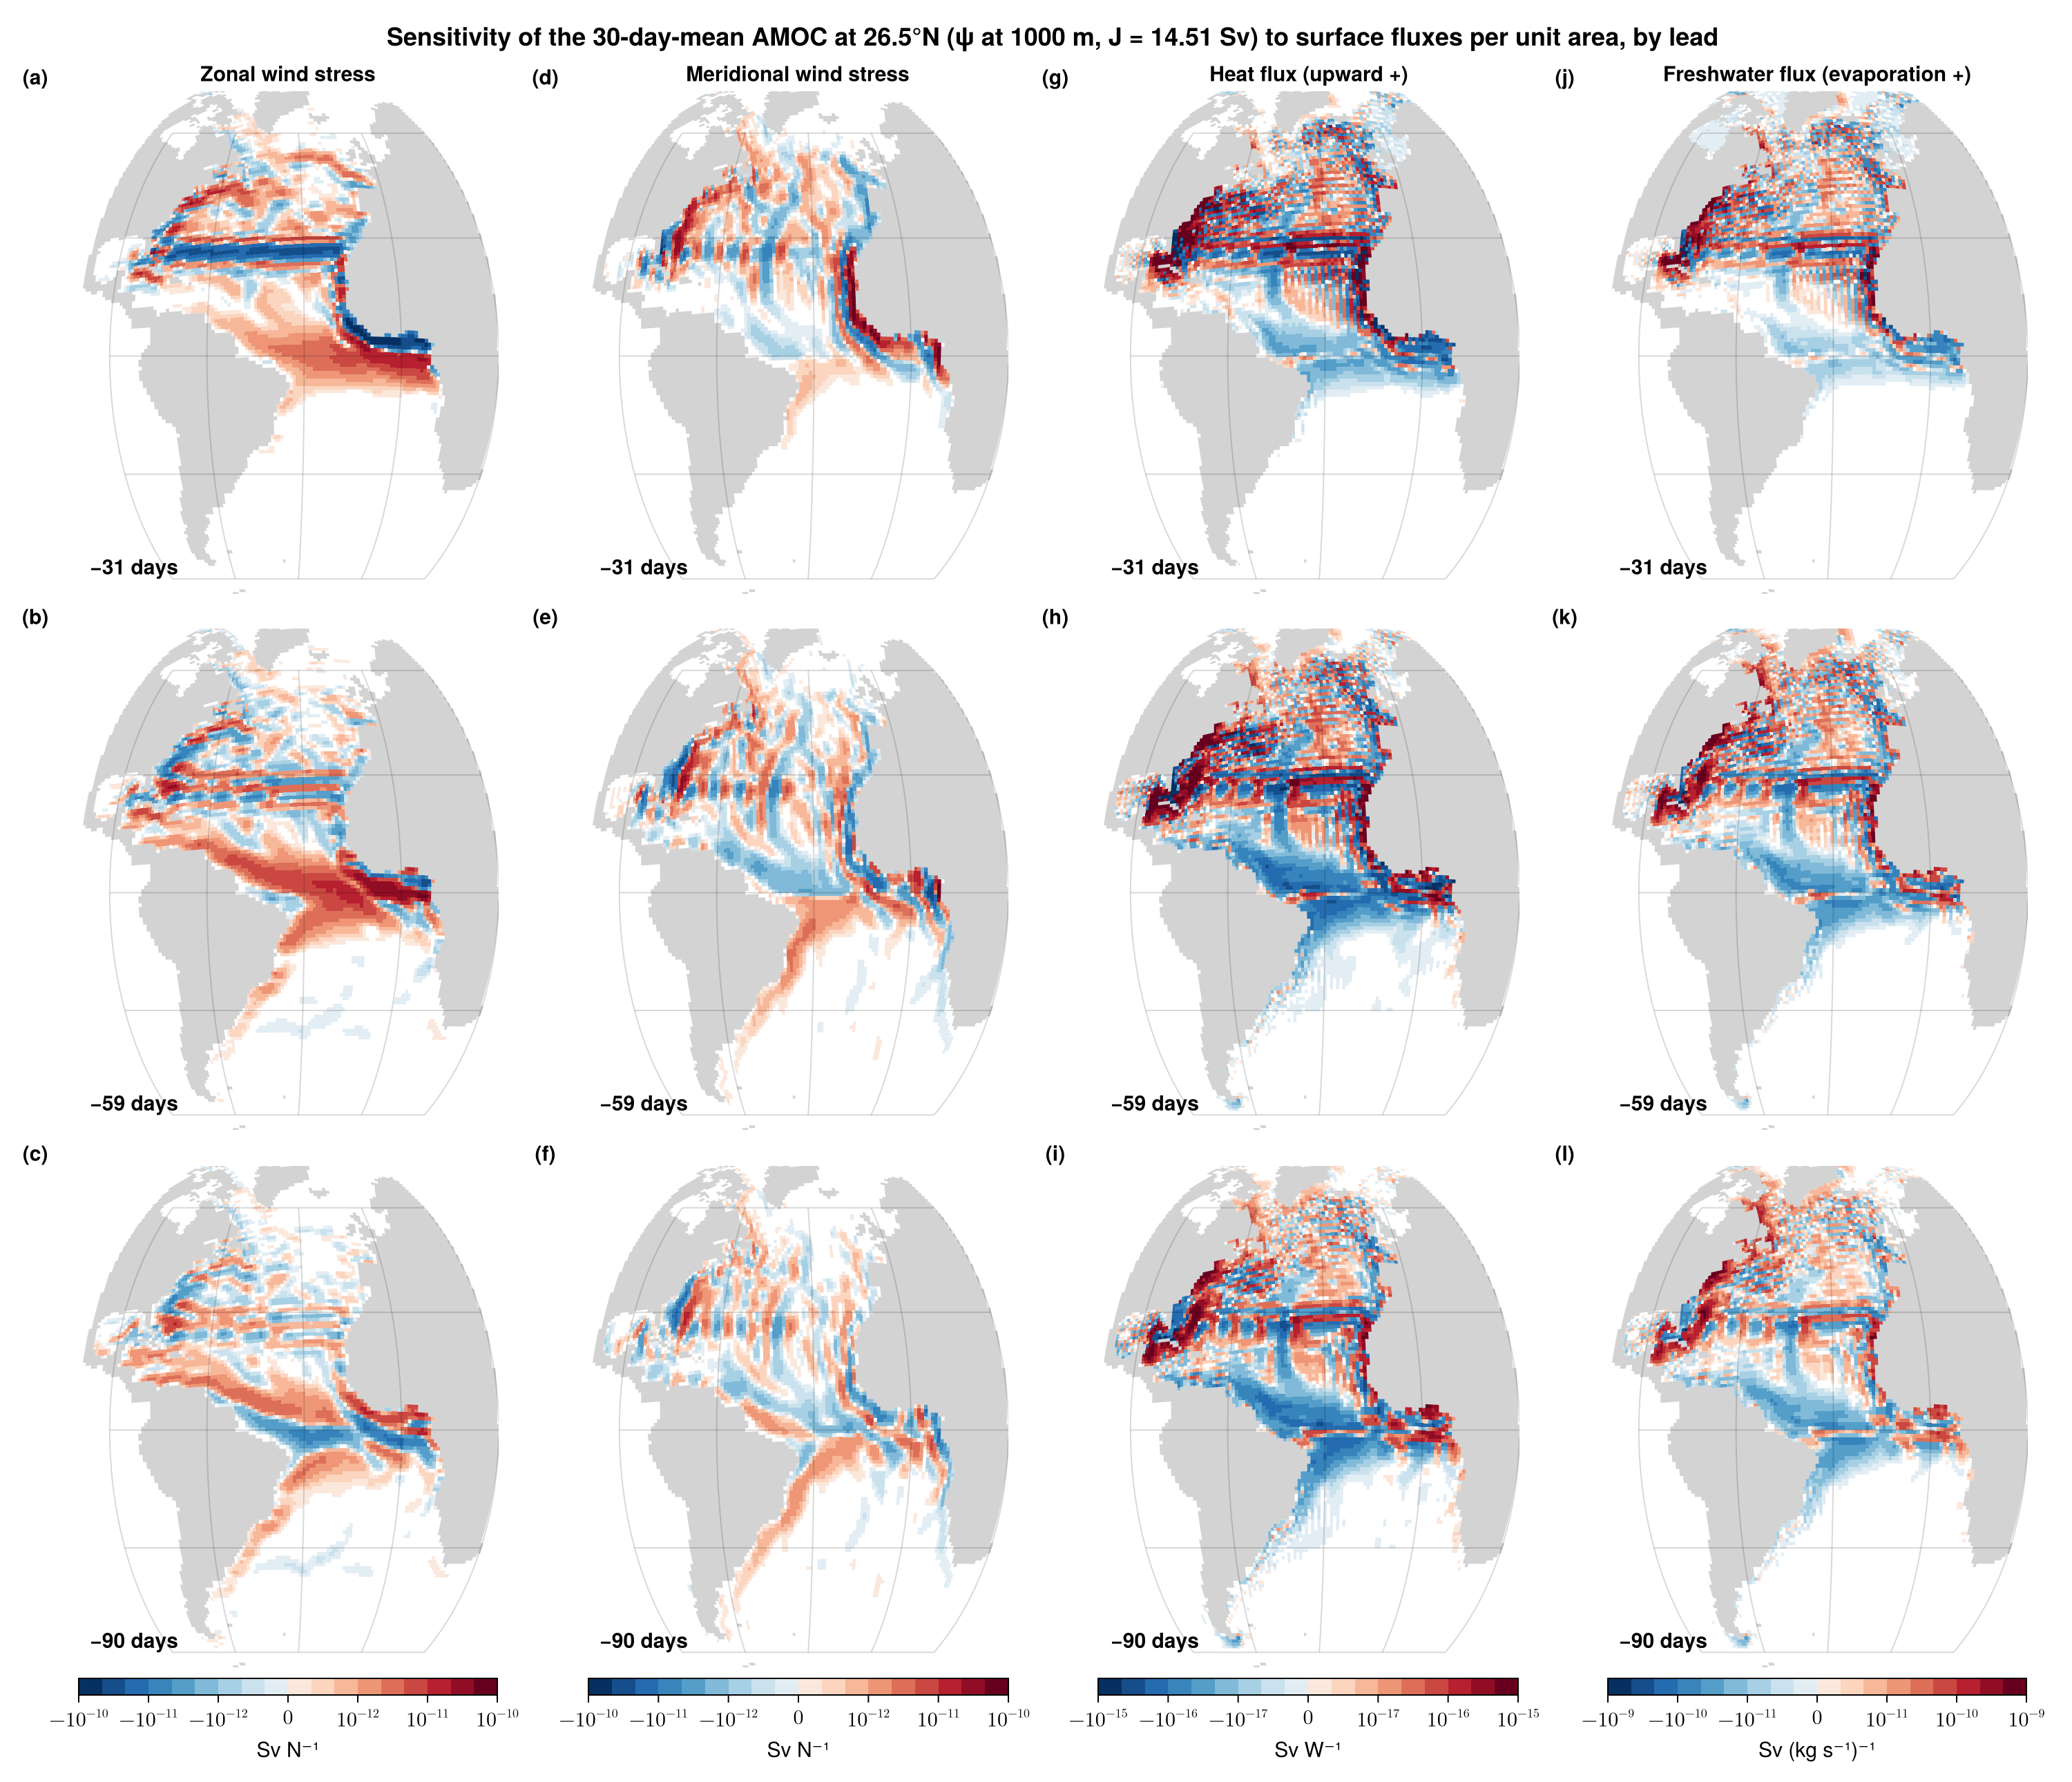
\includegraphics[width=0.8\textwidth]{figures/lead_sensitivity_ecco4_onedegree_nz20_90day_frozen_gradients_upwind3.png}
\caption{Raw sensitivities at \ang{1}, after Pillar et al.\ (2016, Fig.~1). Values are per unit area; positive means
that more eastward or northward stress, more upward heat flux or more evaporation raises the AMOC. Colors are
logarithmic over three decades, and smaller values are white. The heat- and freshwater-flux columns show a
row-to-row stripe over the subpolar North Atlantic interior.}
\label{fig:lead-raw}
\end{figure}

\section{Is the checkerboard real?}

\textbf{Measures.} The \emph{grid-scale share} is the energy in the checker, $i$-stripe and $j$-stripe components of
each $2\times2$ block, divided by the block's total energy. White noise scores 0.75 and a smooth field scores near 0.
The share treats a single spike like noise, so the maps below also use lag-1 correlations $\rho_x, \rho_y$ in
$5\times5$ windows, which separate alternation from spikes. Before any change, heat-flux shares were 0.6--0.9 at
\ang{1} and 0.4--0.9 at \ang{2}. 79--83\,\% of the 100 largest heat-flux sensitivities sat in convecting columns,
which are 16\,\% of the wet columns.

\textbf{Finite differences} along the grid-scale part of the gradient (each check is a central-difference scan
over $h$):

\begin{center}\small
\begin{tabular}{@{}p{0.5\textwidth}lr@{}}
\toprule
Direction & adjoint & FD / adjoint \\
\midrule
\ang{2}, 14 days: flux and stress gradients & frozen CATKE & 0.997--0.999 \\
\ang{2}, 14 days: stress; one heat-flux cell & CATKE differentiated & 0.889; 0.16 \\
\ang{2}, 14 days: grid-scale heat-flux part, never-convecting blocks & frozen CATKE & 0.997 \\
\ang{1}, 90 days: same part, stable blocks; stress & frozen CATKE & $1.00 \pm 0.03$; 1.003 \\
\ang{1}, 90 days: same part, convecting blocks & frozen CATKE & 1.8--3.2 (rough) \\
\bottomrule
\end{tabular}
\end{center}

So the grid-scale flux sensitivity is what the model does. The pieces of the investigation fit together as follows:
\begin{itemize}
  \item \emph{CATKE differentiated.} The adjoint is exact at 8, 42 and 84 steps and wrong at 168. A one-step
        dot-product test localizes the error to step 120: one cell at the mixed-layer base whose TKE is $\num{6e-8}$,
        under its \SI{e-4}{m^2\,s^{-2}} floor, receives a reverse value 60 times its neighbors'.
  \item \emph{Holding TKE fixed in the derivative.} This removes that spike, but convecting directions still come out
        wrong ($-0.19$ to 0.03) because of CATKE's convective and near-neutral switches. No stop-gradient mask fixed
        it.
  \item \emph{Wind stress.} The model interpolates stress from cell centers to faces, so $\partial J/\partial\tau_x$
        has no component alternating in $i$ and $\partial J/\partial\tau_y$ none alternating in $j$ (shares
        0.00--0.04). The heat and freshwater fluxes enter at cell centers and keep all three components.
  \item \emph{Things that are not the cause.} The structure is unchanged with WENO or upwind3 advection, and is as
        noisy with GM/Redi off. Biharmonic tracer diffusion lowers the share only to 0.53--0.73. The \SI{0.26}{K}
        grid-scale residual in forward surface temperature is already in the ECCO4 initial state.
\end{itemize}

\section{Where it lives}

\begin{figure}[H]
\centering
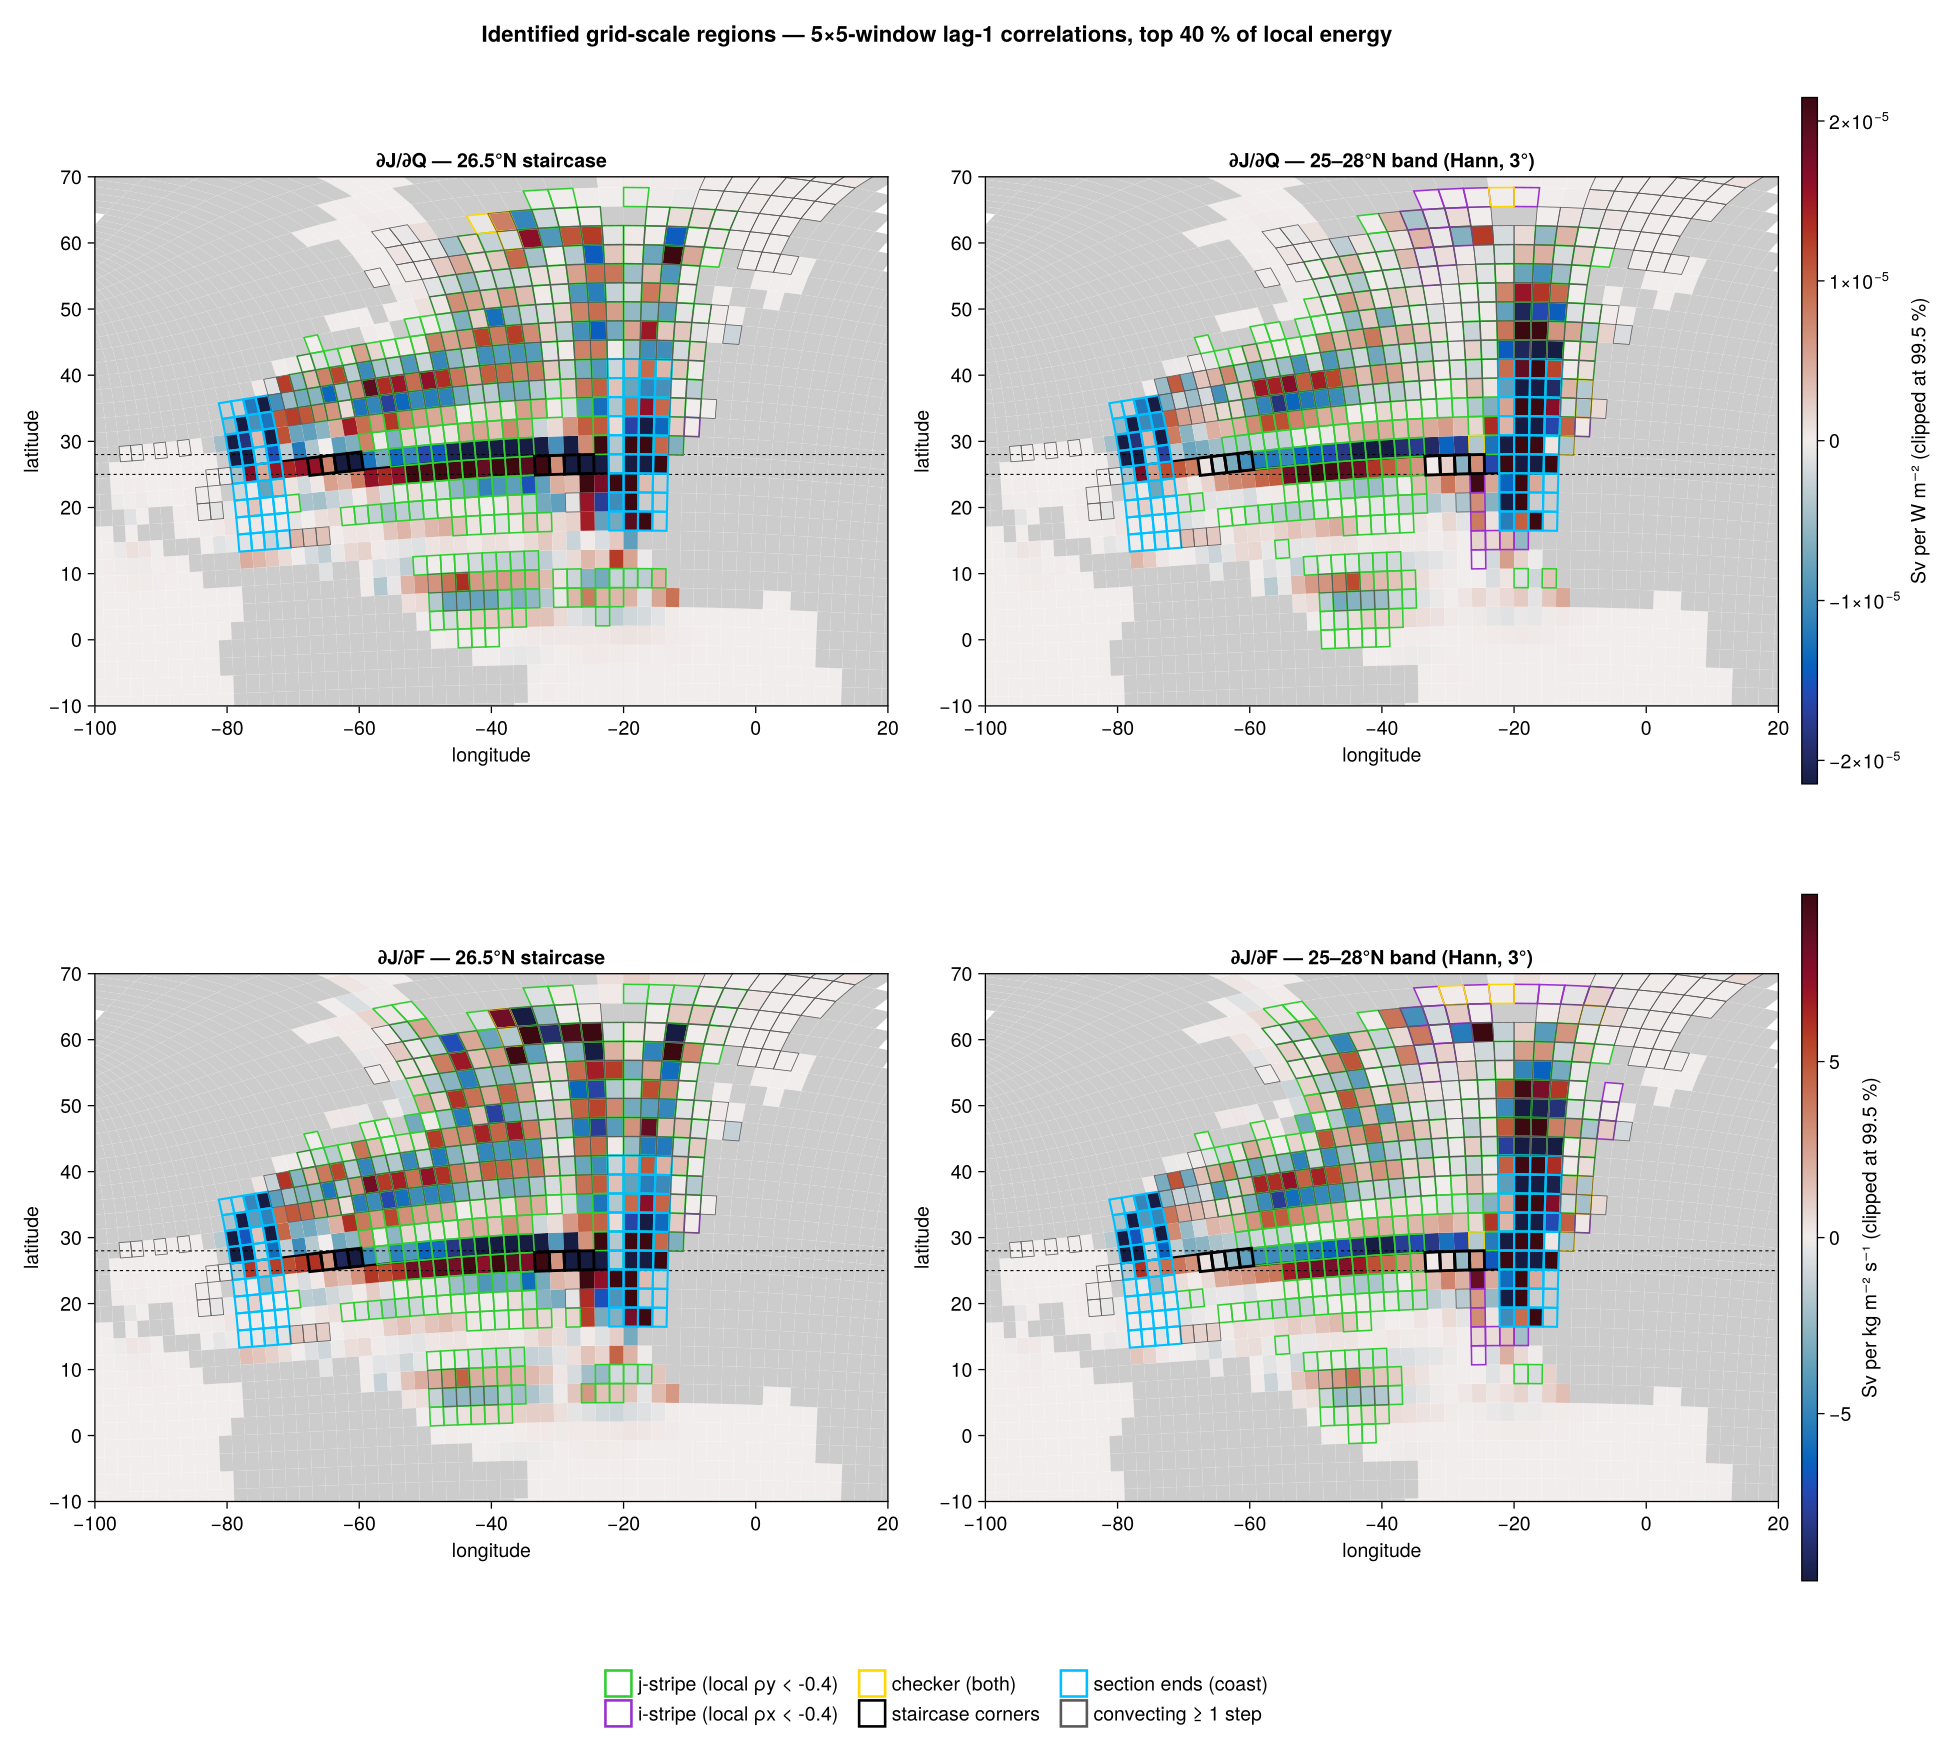
\includegraphics[width=0.84\textwidth]{figures/checkerboard_regions_twodegree_14day_band.png}
\caption{\ang{2}, 14 days, frozen CATKE (1167068); slice-summed heat-flux (top) and freshwater-flux (bottom)
sensitivities. Left: the staircase objective. Right: the objective averaged over a \ang{3} Hann band (1174907). Cells
are outlined where the local $\rho_y$ or $\rho_x$ is below $-0.4$ and the local energy is in the Atlantic's top
\SI{40}{\percent}.}
\label{fig:regions2}
\end{figure}

At \ang{2} (Fig.~\ref{fig:regions2}), 334 heat-flux cells alternate row to row, 1 column to column, and 3 as a
checker. Of the heat-flux energy:
\begin{itemize}
  \item \SI{55}{\percent} is in the coastal cells at the two ends of the section;
  \item \SI{23}{\percent} is in the dipole along the section line;
  \item \SI{13}{\percent} is in convecting columns;
  \item \SI{7}{\percent} is in the staircase corners.
\end{itemize}

\textbf{A band-averaged objective} (prototype, $J = 15.02$ against \SI{15.56}{Sv}) removes the corners and halves
the line's share. It raises the ends' share to 0.78 and leaves the row stripe away from the section unchanged. It is
not a fix.

\begin{figure}[H]
\centering
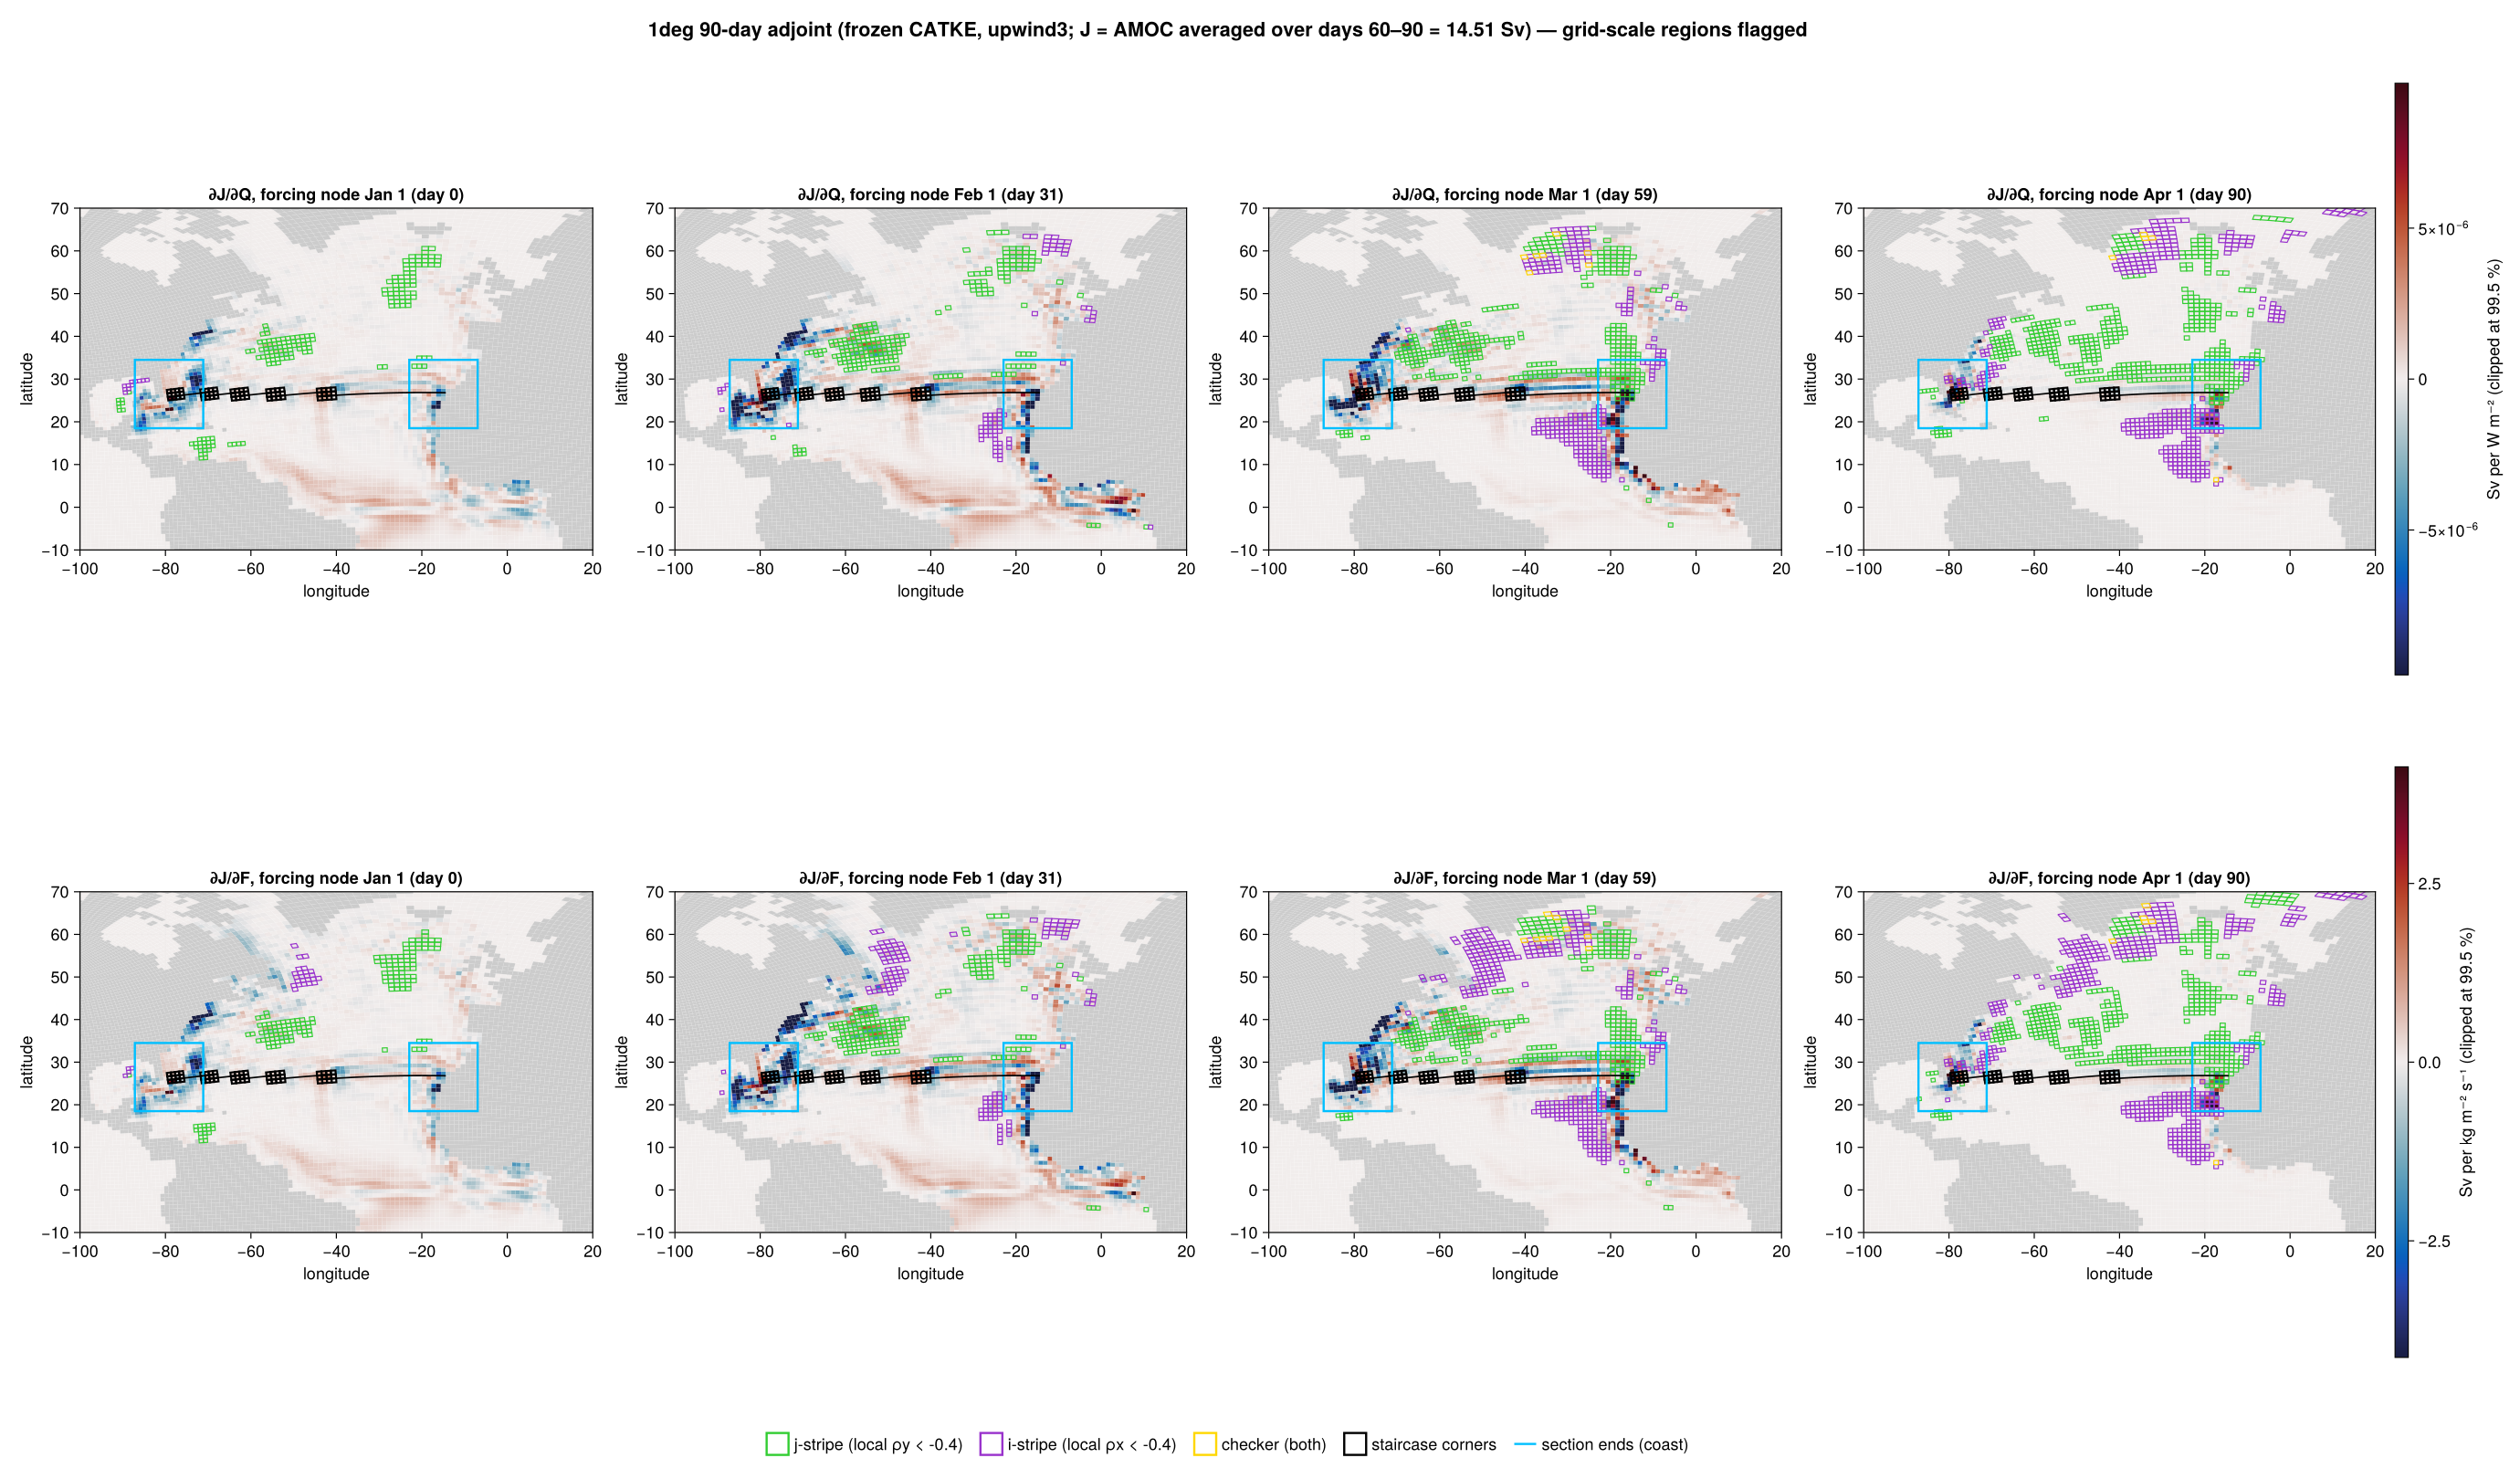
\includegraphics[width=\textwidth]{figures/checkerboard_regions_onedegree_90day.png}
\caption{\ang{1}, 90 days (1161433): heat flux (top) and freshwater flux (bottom) at each forcing node, outlined as in
Fig.~\ref{fig:regions2}. Black: the staircase corners. Blue boxes: the section's coastal ends.}
\label{fig:regions1}
\end{figure}

At \ang{1} (Fig.~\ref{fig:regions1}) the corners and coastal ends hold \SI{91}{\percent} of the last slice's
heat-flux energy, in paths one or two cells wide:
\begin{itemize}
  \item the Florida Straits and the Gulf Stream to \ang{42}N;
  \item the African coast to the equator and the Gulf of Guinea.
\end{itemize}
These paths are boundary-wave pathways and are physically expected.

\textbf{The stripe.} Averaged over the basin, \ang{1} shows no row stripe ($\rho_y = +0.44$ to $+0.66$). In the
North Atlantic interior box of Fig.~\ref{fig:box} (\ang{60}--\ang{10}W, \ang{30}--\ang{65}N), however:
\begin{itemize}
  \item it is present at leads of 31 and 59 days ($\rho_y = -0.37$, $-0.30$) with share 0.62--0.78;
  \item \SIrange{91}{98}{\percent} of the box's energy is in convecting columns, which are 81\,\% of its cells;
  \item the box holds only \SIrange{1}{4}{\percent} of the Atlantic's energy, at \SIrange{4}{19}{\percent} of its peak.
\end{itemize}
The stripe therefore sits exactly where the frozen-CATKE adjoint was found to be biased.

\textbf{Unexplained, \ang{1} only:} a column-to-column stripe at \ang{5}--\ang{24}N, \ang{20}--\ang{45}W, west of
the African coastal column, in the Mar and Apr slices (purple in Fig.~\ref{fig:regions1}; about \SI{10}{\percent} of
the coastal peak).

\section{Smoothed flux controls}

The heat and freshwater fluxes are written as $Q = Q_0 + S c$:
\begin{itemize}
  \item $S$ is a number of passes of a 1-2-1 average, first in $i$ (periodic), then in $j$, over wet--wet edges
        only, closed at the southern boundary and the fold.
  \item The gradient with respect to the controls is $\partial J/\partial c = S^{\mathsf T}\gvec$.
  \item It is applied after the adjoint, so it costs nothing and is exact in $c$. The dot test
        $\langle Sx, y\rangle = \langle x, S^{\mathsf T}y\rangle$ holds to \num{5.5e-15}.
  \item A descent step in the fluxes is $\Delta Q = -\alpha\, S S^{\mathsf T}\gvec$.
\end{itemize}
The finite-difference stage moves along $S d$ when smoothing is on.

\begin{center}\small
\begin{tabular}{@{}lcccc@{}}
\toprule
Grid-scale share of $\partial J/\partial Q$ & raw & 1 pass & 2 passes & $\partial J/\partial\tau_x$ \\
\midrule
\ang{2}, 14 days (by latitude band) & 0.58--0.96 & 0.24--0.56 & 0.12--0.31 & 0.28--0.84 \\
\ang{1}, 90 days (by latitude band) & 0.17--0.92 & 0.07--0.52 & 0.04--0.29 & 0.06--0.45 \\
\ang{1}, interior box of Fig.~\ref{fig:box} & 0.62--0.78 & 0.22--0.24 & 0.11--0.12 & -- \\
\bottomrule
\end{tabular}
\end{center}
With two passes the flux sensitivities are as smooth as the stress's. In the box, $\rho_y$ goes from negative to
$+0.86$.

\begin{figure}[H]
\centering
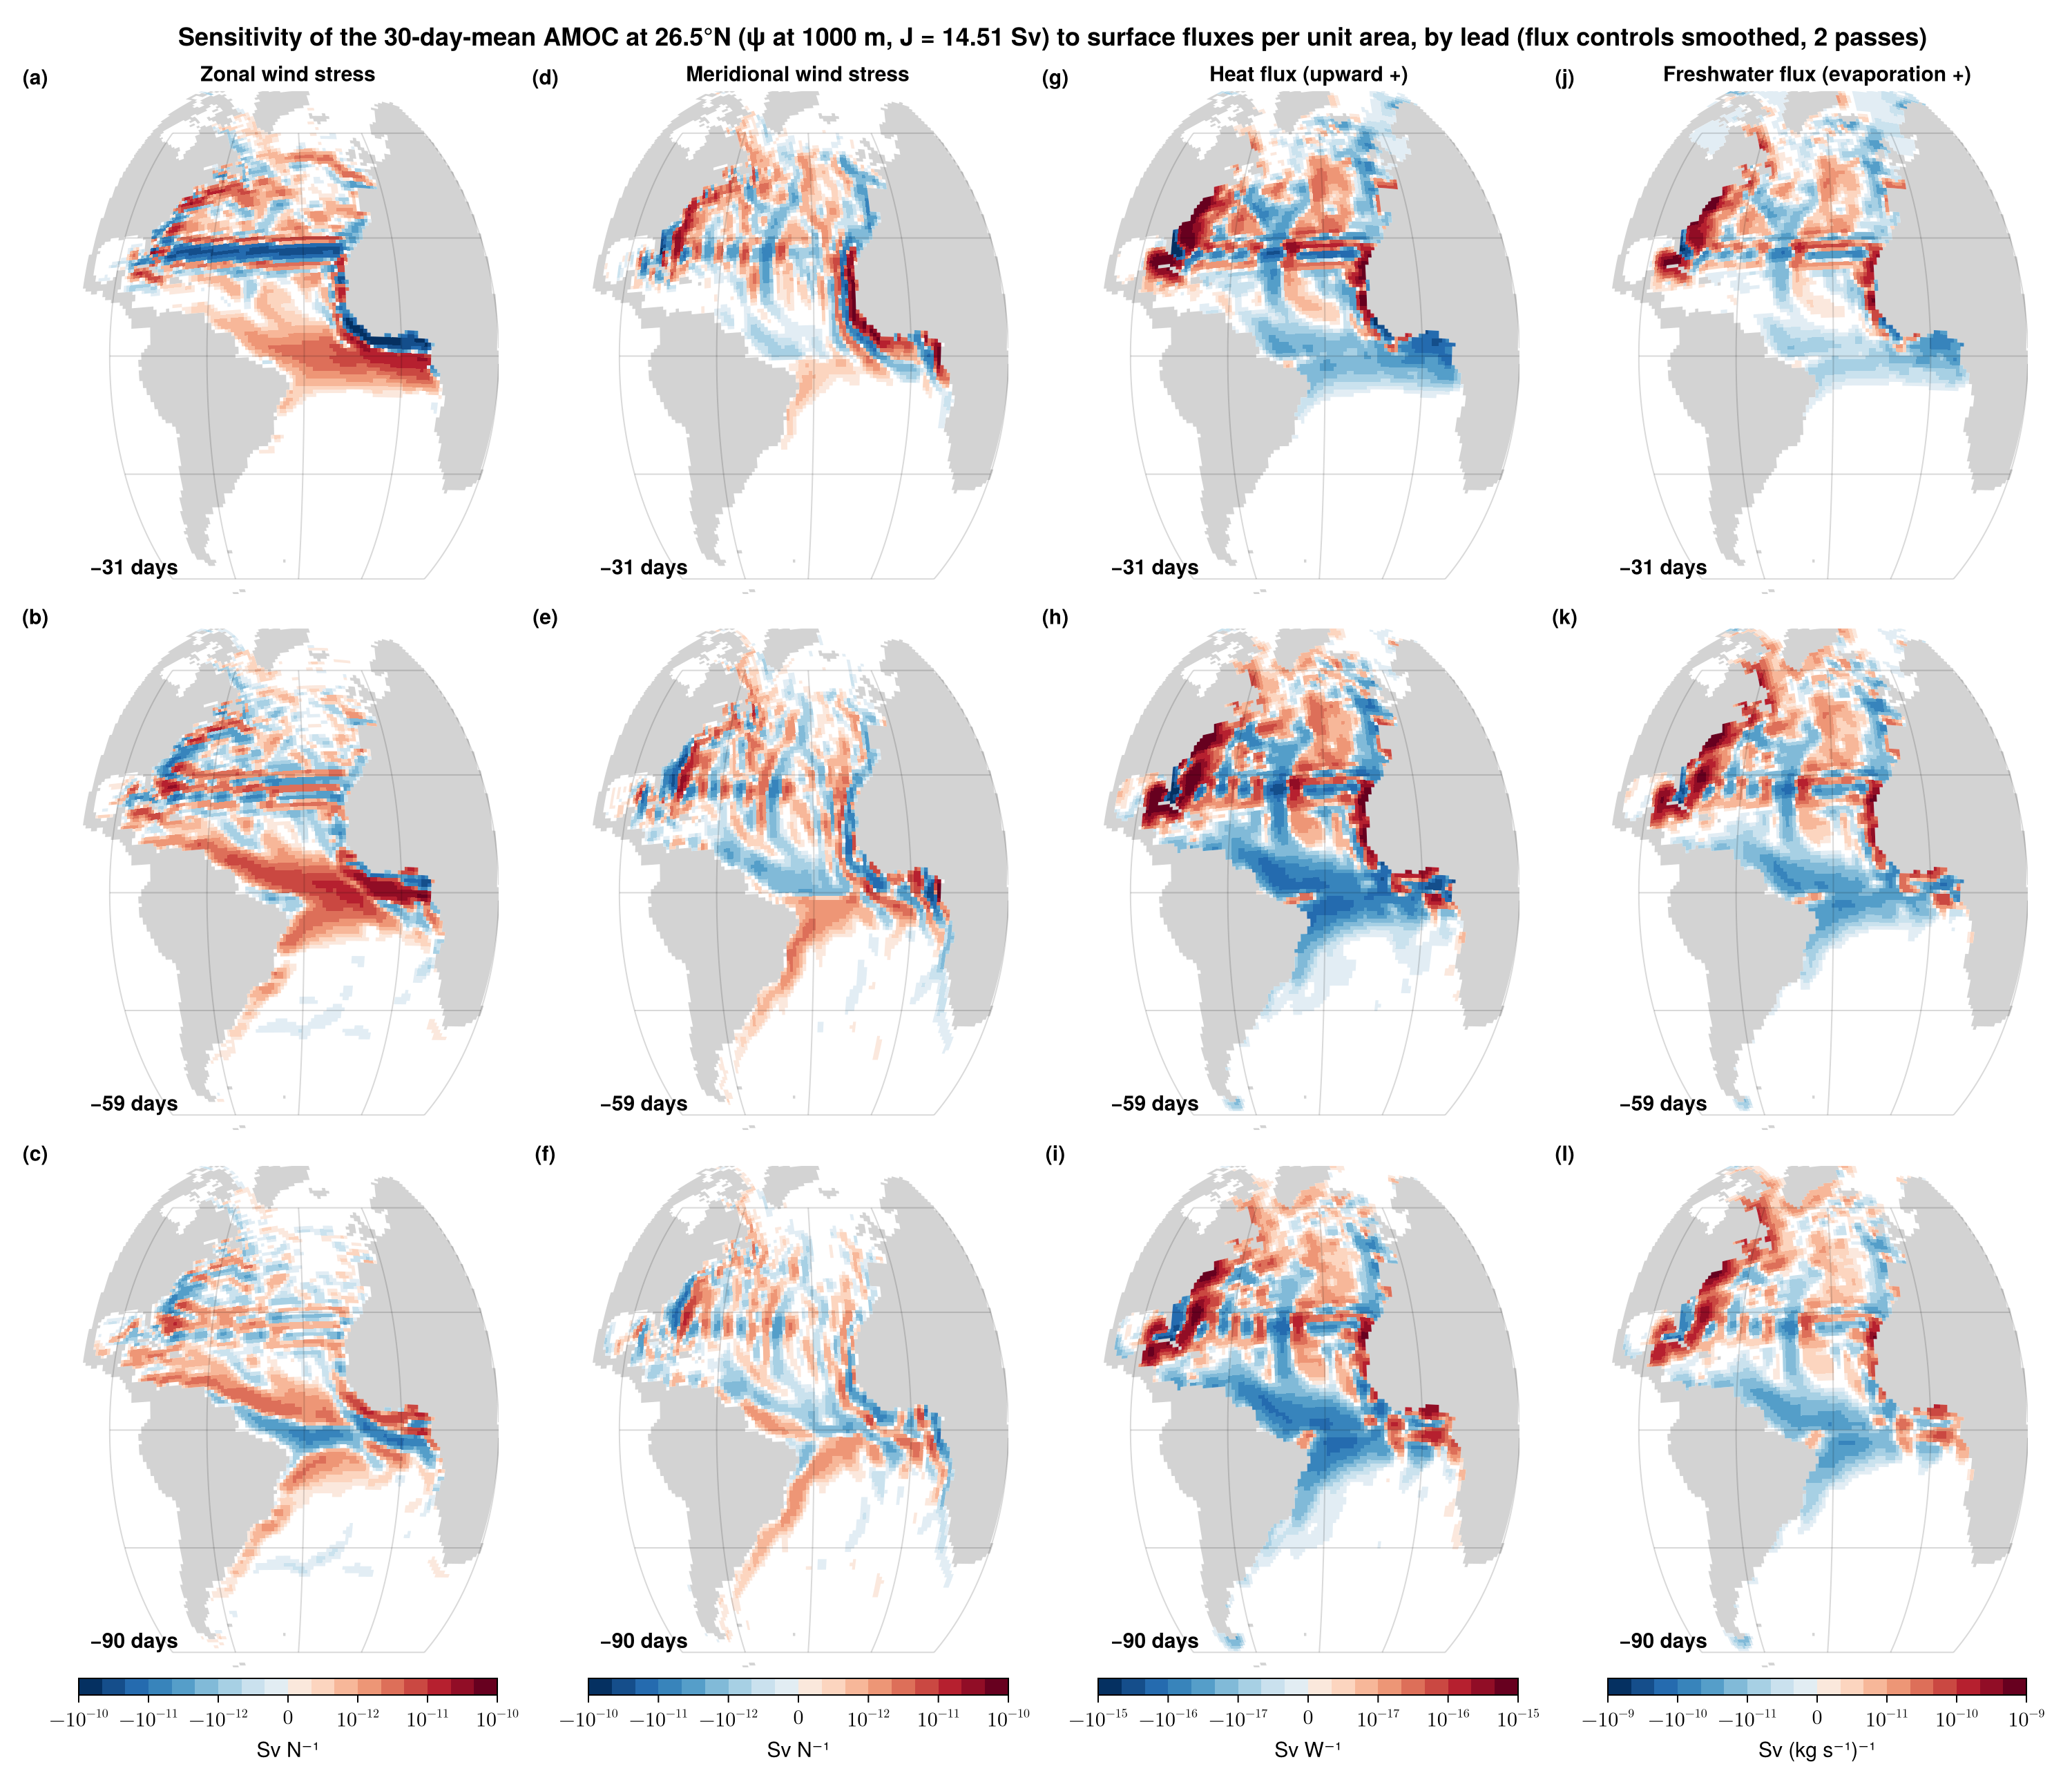
\includegraphics[width=0.8\textwidth]{figures/lead_sensitivity_ecco4_onedegree_nz20_90day_frozen_gradients_upwind3_smoothed2.png}
\caption{As Fig.~\ref{fig:lead-raw}, with the flux columns given as sensitivities to the smoothed controls
($S^{\mathsf T}\gvec$, 2 passes). The stress columns are unchanged.}
\label{fig:lead-smooth}
\end{figure}

\textbf{What the smoothed maps show} (Fig.~\ref{fig:lead-smooth}). The heat- and freshwater-flux columns share one
pattern at every lead:
\begin{itemize}
  \item positive along the western boundary from the Gulf of Mexico to the Labrador Sea, along the African coast, and
        over a patch of the eastern subpolar interior: more upward heat flux or more evaporation there raises the AMOC;
  \item negative over the tropical and South Atlantic;
  \item a band of alternating sign along the section, and north--south bars south of it. I have not yet checked
        whether those bars line up with the steps of the \ang{1} staircase.
\end{itemize}

\begin{figure}[H]
\centering
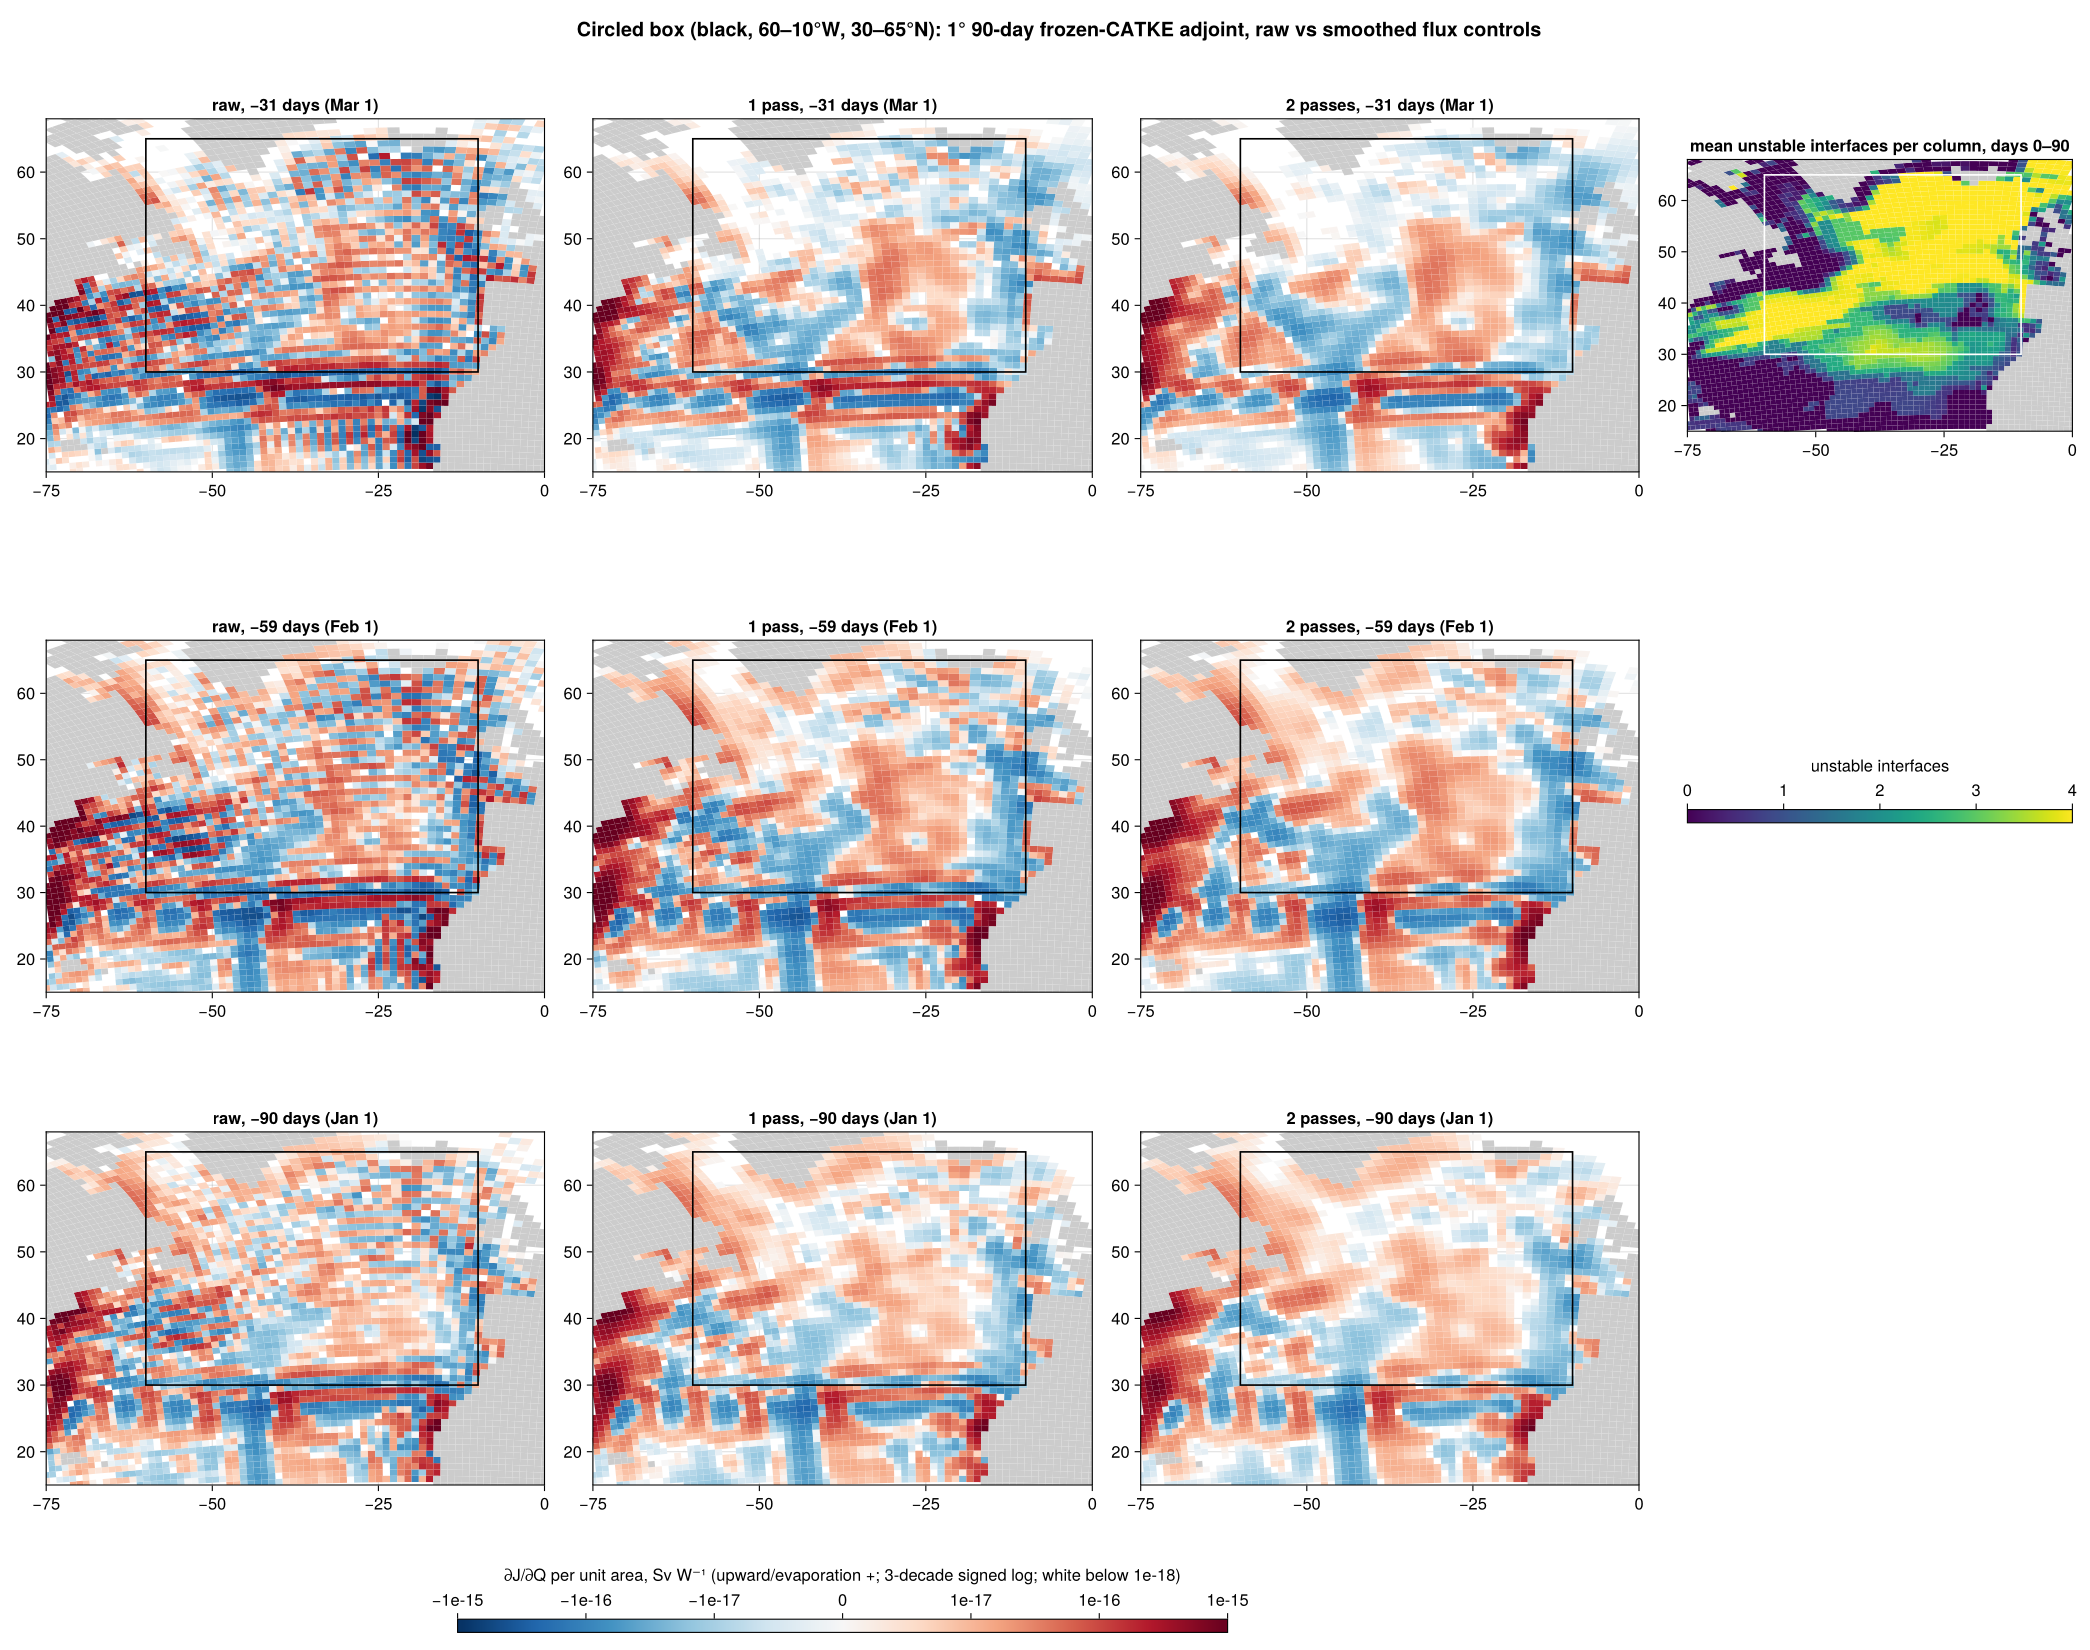
\includegraphics[width=0.9\textwidth]{figures/smoothing_box_heat_onedegree_90day.png}
\caption{The North Atlantic interior (box, \ang{60}--\ang{10}W, \ang{30}--\ang{65}N): heat-flux sensitivity per unit
area, raw and after 1 and 2 passes, at the three leads, colored as in Fig.~\ref{fig:lead-raw}. Top right: mean
number of statically unstable interfaces per column over the window. The raw row stripe covers the convecting
region.}
\label{fig:box}
\end{figure}

\section{Error bars for the smoothed controls}

Smoothing does not change the bias of the frozen-CATKE adjoint in convecting columns; it only weights directions
differently. We therefore checked the directions an optimization with smoothed controls would actually follow. Each
direction is the 2-pass smoothed gradient restricted to a box and to one set of columns, where \emph{convecting} means
at least one unstable interface on average over the window and \emph{stable} means none. Each was scanned over six
halvings of $h$ (ChkFDSm2, 1175918, \SI{57}{min} on one GH200).

\begin{center}\small
\begin{tabular}{@{}lccc@{}}
\toprule
Direction & central FD / adjoint, best $h$ & range over the six $h$ & error bar \\
\midrule
Heat flux, convecting columns \ang{30}--\ang{70}N & 1.04, 1.04 & 0.92--1.46 & $\pm\SI{10}{\percent}$ \\
Heat flux, stable columns \ang{18}--\ang{70}N & 1.03 (smallest $h$) & 1.03--3.1 & $\pm\SI{10}{\percent}$ \\
Heat flux, Labrador Sea & 0.98; backward side 1.00--1.07 at every $h$ & 0.69--1.53 & $\pm\SI{5}{\percent}$ \\
Heat flux, eastern subpolar gyre & not converged & 0.89--1.23 & $\pm\SI{25}{\percent}$ \\
Freshwater flux, convecting columns & 0.99, 0.94, 0.89 & $-2.2$--1.22 & $\pm\SI{10}{\percent}$ \\
Freshwater flux, stable columns & 0.93 (smallest $h$) & 0.93--3.5 & $\pm\SI{10}{\percent}$ \\
\bottomrule
\end{tabular}
\end{center}

\begin{figure}[H]
\centering
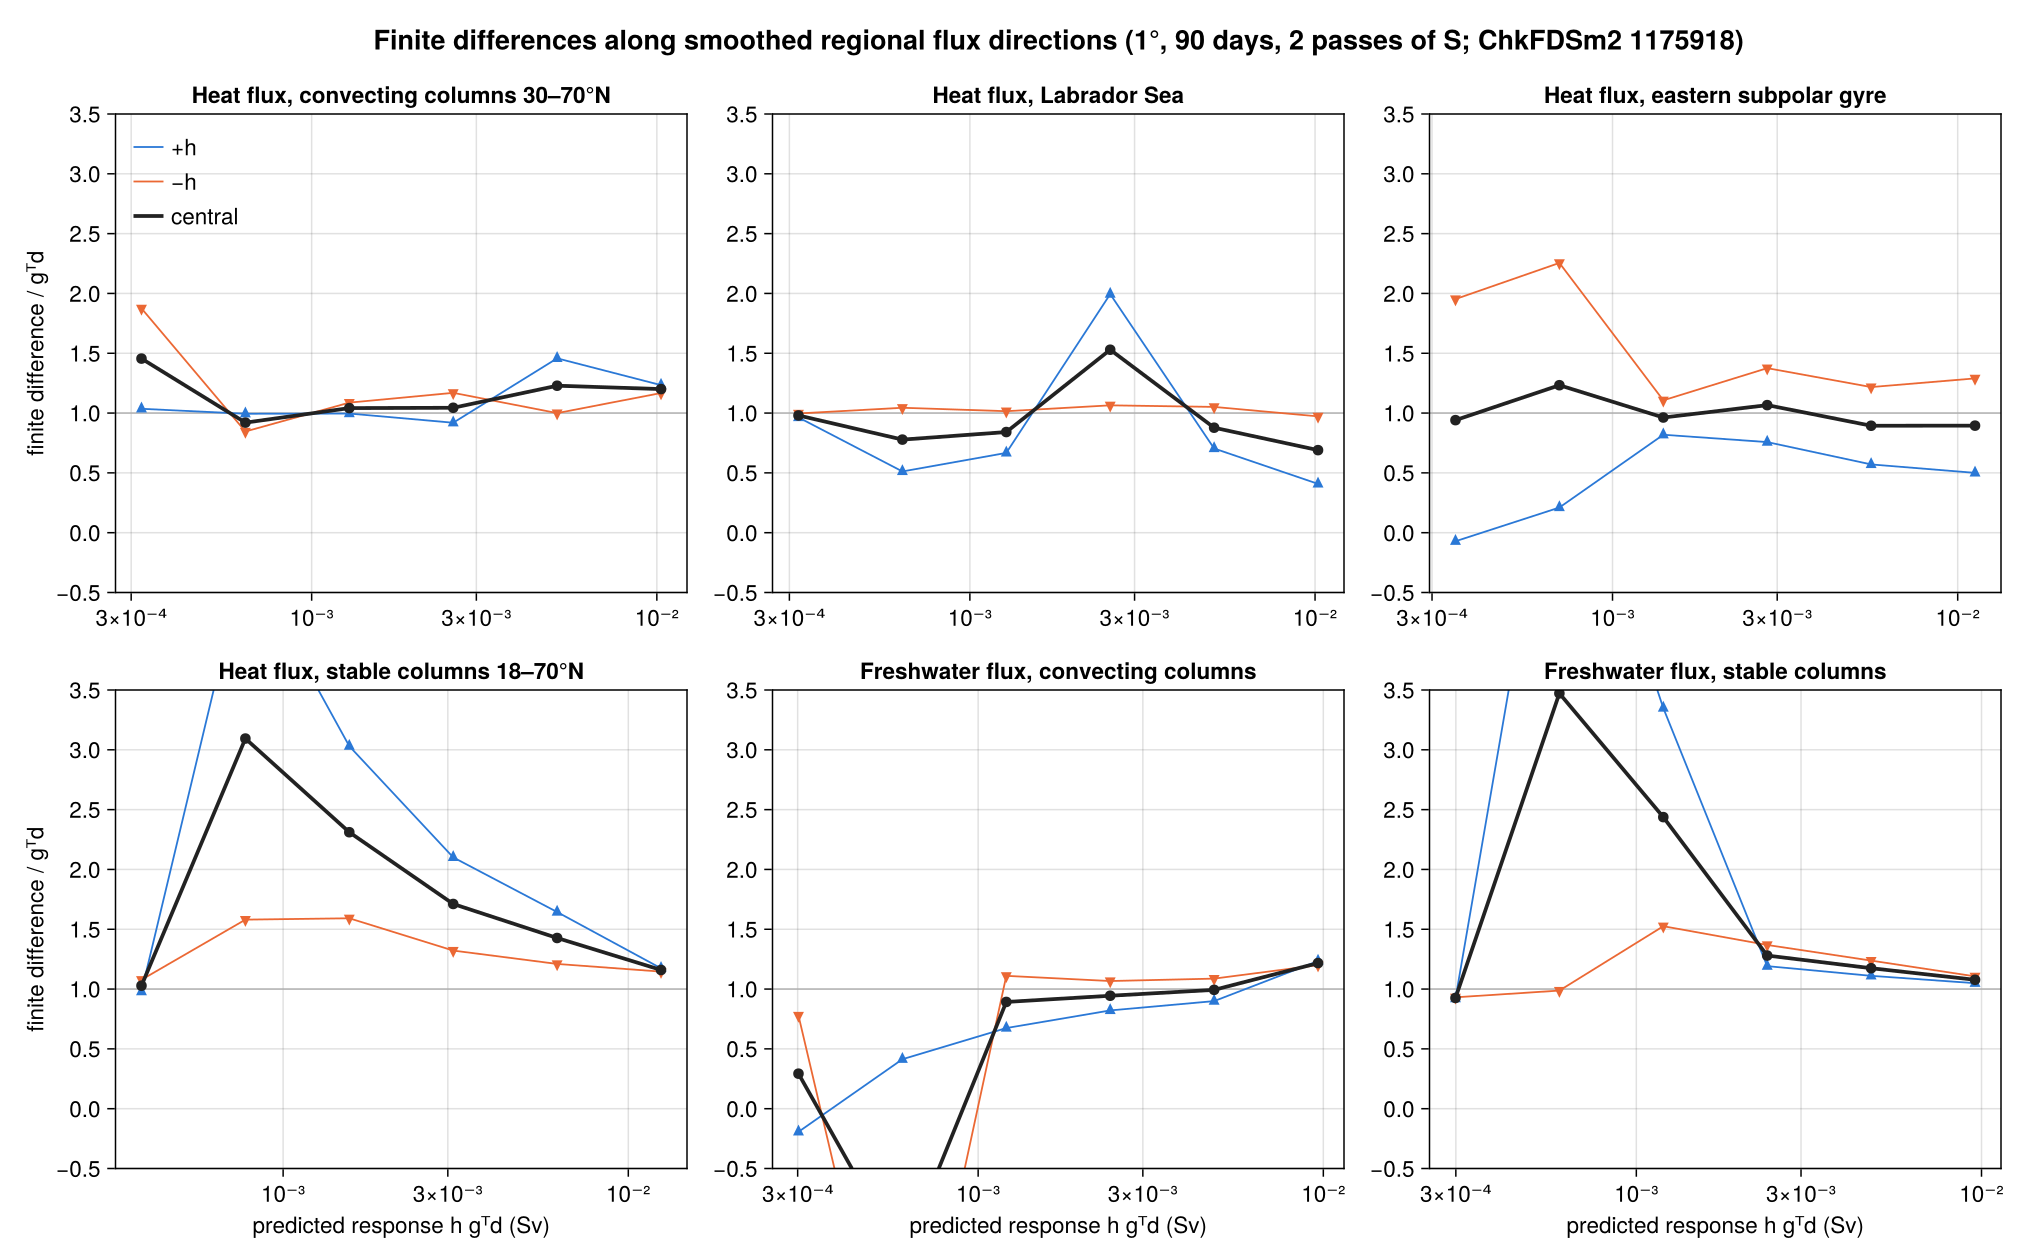
\includegraphics[width=0.9\textwidth]{figures/fd_directions_onedegree_90day_upwind3_smoothed2.png}
\caption{Forward ($+h$), backward ($-h$) and central differences divided by the adjoint's $\gvec^{\mathsf T}d$, against
the predicted response $h\,\gvec^{\mathsf T}d$. A switch in the forward model moves one side away from 1 while the other
stays.}
\label{fig:fd}
\end{figure}

\textbf{The scatter is discrete, not curvature} (Fig.~\ref{fig:fd}):
\begin{itemize}
  \item Single perturbed runs land \SIrange{e-4}{4e-3}{Sv} off the linear response, with either sign and at no
        consistent $h$. In the stable directions this happens at every $h$ except the smallest.
  \item These jumps are the CATKE switches of the live forward model, the same piecewise smoothness reported last
        time. They are as large as the response at the small steps, so they set the error bars.
  \item The cleanest case is the Labrador Sea: its backward differences stay at 1.00--1.07 at every $h$, while the
        forward side jumps.
\end{itemize}

The roughly 2$\times$ bias in convecting columns was measured along their grid-scale part (1.8--3.2), and along a single
smoothed cell the ratio was 0.86. Neither appears along region-wide smoothed directions. The bias is confined to
grid-scale and single-cell directions, which the smoothed controls do not follow.

\section{Next steps and decisions}

\begin{enumerate}
  \item \textbf{Decided:} the frozen-CATKE adjoint with two-pass smoothed flux controls, for the lead-time maps and
        for flux optimization. A convective-mixing scheme used only in the adjoint is set aside.
  \item The band-averaged objective stays a prototype. If the section's corners matter for a figure, it removes them.
  \item Open, \ang{1} only: the column-to-column stripe west of Africa, and whether the bars south of the section in
        Fig.~\ref{fig:lead-smooth} follow the staircase steps.
  \item Separate issue: for the GM/Redi coefficients the frozen adjoint gives 0.25--0.6 of the $\kappa_{\text{skew}}$
        slope. With two parameters, central differences are exact and cheaper (\SI{36}{s} against \SI{93}{s} at
        90 days), so calibration does not need the adjoint.
  \item Then, as before: longer windows (the 1-year burst at \ang{63}W \ang{61}S), a spun-up initial state, and
        one-year lead maps after Pillar et al.
\end{enumerate}

\end{document}
